\subsection{Definition}

In addition to the previous example (section \ref{bmt:heat_transport_fracture}) now we consider heat transport in a two-phase homogeneous porous medium consisting of a solid and liquid phase, i.e. a 1D test example for groundwater flow and simultaneous heat transport in an aquifer. The aim of the numerical simulation is also to determine the effect of varying density value with temperature changes. 
%

\subsection{Solution}

For the 1-dimensional calculation the calculation area is simplified as a line of a length of $\unit[5.2]{m}$. The calculation model includes 25 elements and 26 nodes. The initial pressure in the whole area is $\unit[100]{kPa}$ and the initial temperature $\unit[300]{K}$. As boundary condition a constant pressure of $\unit[101]{kPa}$ is given at the left boundary and of $\unit[100]{kPa}$ at the right boundary. A constant temperature of $\unit[400]{K}$ is set at the left boundary. The used soil parameters are listed in Tab.~\ref{tab41}. The fluid density is decreasing with increasing temperature. The viscosity, capacity and conductivity of water are set to constant values. The fluid parameters also can be found in Tab.~\ref{tab41}.

\begin{table}[htbp]
\caption{\label{tab41}Used soil and fluid parameters.}
\begin{center}
\begin{tabular}{llrr}
\toprule
Symbol & Parameter & Value & Unit \\
\midrule
\multicolumn{2}{c}{\textit{Soil parameters}}\\
$\phi$ & Porosity & 0.01 & - \\	
$k$ & Permeability & $\unit[1.0 \cdot 10^{-11}]{}$ & ${m^{2}}$ \\
$\rho^s$ & Density & $\unit[2850]{}$ & ${kg \cdot m^{-3}}$ \\
$c^s$ & Heat capacity	& $\unit[1000]{}$ & ${J \cdot kg^{-1} \cdot K^{-1}}$ \\
$\lambda^s$	& Heat conductivity & $\unit[3.2]{}$ & ${W \cdot m^{-1} \cdot K^{-1}}$ \\
\cmidrule{1-2}
\multicolumn{2}{c}{\textit{Fluid parameters}}\\
$\rho^f_0$ & Initial density & $\unit[1000]{}$ & ${kg \cdot m^{-3}}$ \\
$\eta$ & Viscosity & $\unit[0.001]{}$ & ${N \cdot s \cdot m^{-2}}$ \\
$c^f$ & Heat capacity	& $\unit[4000]{}$ & ${J \cdot kg^{-1} \cdot K^{-1}}$ \\
$\lambda^f$	& Heat conductivity & $\unit[0.6]{}$ & ${W \cdot m^{-1} \cdot K^{-1}}$ \\
\bottomrule
\end{tabular}
\end{center}
\end{table}

In order to find out whether the consideration of varying water density with temperature changes is possible, one simulation run is done with a constant density of $\unit[1000]{kg/m^{3}}$, which is the initial water density before heating, and one run with a constant density of $\unit[900]{kg/m^{3}}$, the density after the heating process. The temperature results for a heat transport with varying density have to be in between both temperature envelopes.

\subsection{Results}

The curve for temperature evolution, which is shown in Fig.~\ref{figHT1} for the right boundary (node 26), shows the expected characteristics. Therefore it can be stated, that the consideration of temperature dependent fluid density is possible.

\begin{figure}[htbp]
\centering
\includegraphics[width=0.8\textwidth]{PART_II/T/figHT1.eps}
\caption{\label{figHT1}Temperature evolution with constant and variable fluid densities.}
\end{figure}
